\documentclass[12pt]{exam}
\usepackage{amsthm}
\usepackage{libertine}
\usepackage[utf8]{inputenc}
\usepackage[margin=1in]{geometry}
\usepackage{amsmath,amssymb}
\usepackage{multicol}
\usepackage[shortlabels]{enumitem}
\usepackage{siunitx}
\usepackage{cancel}
\usepackage{graphicx}
\usepackage{pgfplots}
\usepackage{listings}
\usepackage{tikz}
\usepackage{color, colortbl}
\usepackage{amsbsy}
\usepackage{pgfplots}
\usepackage{caption}
\usepackage{subcaption}
\usepackage{algorithm}
\usepackage{algpseudocode}
\usepackage[]{cancel}


\pgfplotsset{compat=1.11}
\usetikzlibrary{calc}
\pgfplotsset{width=10cm,compat=1.9}
\usepgfplotslibrary{external}
\tikzexternalize
\graphicspath{ {./images/} }

\newcommand{\class}{High Performance Computing 1} % This is the name of the course 
\newcommand{\examnum}{Assignment 1: Write Up} % This is the name of the assignment
\newcommand{\examdate}{\today} % This is the due date
\newcommand{\timelimit}{}





\begin{document}
\pagestyle{plain}
\thispagestyle{empty}

\noindent
\begin{tabular*}{\textwidth}{l @{\extracolsep{\fill}} r @{\extracolsep{6pt}} l}
\textbf{\class} & \textbf{Name:} & \textit{Denzel Ayala}\\ %Your name here instead, obviously 
\textbf{\examnum} &&\\
\textbf{\examdate} &&\\
\end{tabular*}\\
\rule[2ex]{\textwidth}{2pt}
% ---


    \section*{\label{sec:prob1} Problem 1}

        For the fourth part of this problem I obtained all the residues from the provided output file. For the cumulative run time I used a for loop in \textbf{\textit{awk}} to add up all the provided times in the second to last column. In the case of count I gave two possible values. The first was the total number of rows extracted from the original file. The second count given was the addition of all the residues. Below is an image containing the commands I entered as well as the contents of the files requested. My code is slightly different from what is being displayed. For the screenshot I limited the residues gotten by grep using \textit{\ldots(002)}. In the submitted code every residue is printed to the file and the output count and runtime reflect that. 

        \begin{center}
            \includegraphics*[scale=0.4]{prob1.jpg}
        \end{center}

    \section*{\label{sec:prob2} Problem 2}

        \begin{enumerate} %You can make lists!

            \item \textbf{Specify Problem Requirements}

            The goal is to plot the Mandelbrot set by calculating series convergence (eq~\ref{eq:1}) at every point in a space. For this problem we will be working with complex numbers. They consist of a real and \textit{imaginary} component. These two components are orthogonal to each other. As a result the real and imaginary components can be treated as an $\hat{x}$ and $\hat{y}$ axis, respectively.
            \begin{center}
                \begin{gather}\label{eq:1}
                    z_{i} = z^{2}_{i-1} + c
                \end{gather}
            \end{center}

                 We are plotting within a range of $-2 \leq x \leq 2$ and $-1 \leq y \leq 1$. The plot range will be divided into individual points, that I will call \textbf{\textit{pixels}}, where convergence is tested. The ordered combination of the pixels form a mesh that determines the resolution power of the calculation. The plot on the left would be a representation of a low resolution mesh while on the left is a high resolution mesh. 

                 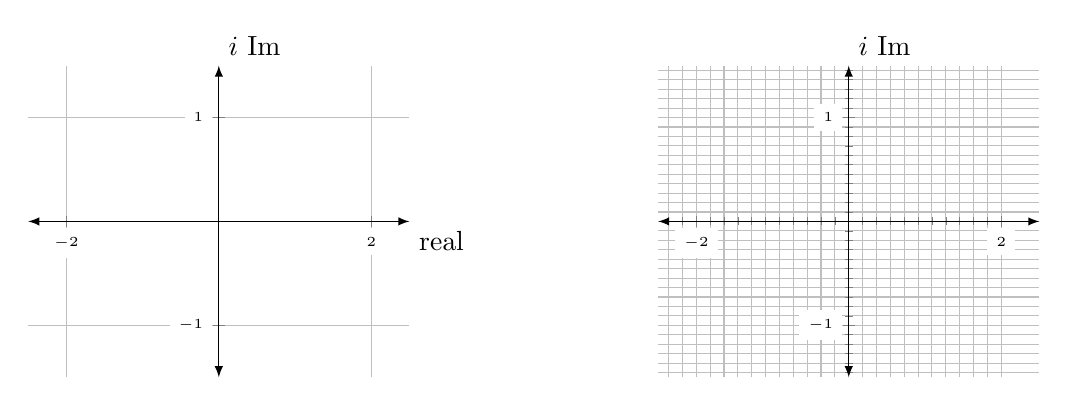
\begin{tikzpicture}
                    \begin{axis}[
                        xmin=-2,xmax=2,
                        ymin=-1,ymax=1,
                        grid=both,
                        axis lines=middle,
                        minor tick num=0,
                        enlargelimits={abs=0.5},
                        axis line style={latex-latex},
                        ticklabel style={font=\tiny,fill=white},
                        xlabel style={at={(ticklabel* cs:1)},anchor=north west},
                        ylabel style={at={(ticklabel* cs:1)},anchor=south west},
                        xlabel={real}, ylabel={$i$ Im},
                        width={0.55*\textwidth-7pt}
                    ]                   
                    \end{axis}
                
                    \begin{axis}[xshift=8cm,
                        xmin=-2,xmax=2,
                        ymin=-1,ymax=1,
                        grid=both,
                        axis lines=middle,
                        minor tick num=10,
                        enlargelimits={abs=0.5},
                        axis line style={latex-latex},
                        ticklabel style={font=\tiny,fill=white},
                        xlabel style={at={(ticklabel* cs:1)},anchor=north west},
                        ylabel style={at={(ticklabel* cs:1)},anchor=south west},
                        ylabel={$i$ Im},
                        width={0.55*\textwidth-7pt}
                    ]
                    \end{axis}
                \end{tikzpicture}
                    
                
                The convergence condition at a given pixel is $|z|\leq 2$. For understandability, an iteration will be a singular calculation of equation (\ref{eq:1}), where $z_i$ is the output of each iteration. A round will consist of iteration till divergence or assumed convergence after 1k-10k iterations. For the first iteration of each round $z_{i-1} = z_0 = 0$. Meanwhile, $c$ is given by the plot location of each pixel, or more tangibly each intersection (or square) in the plots above.

                The area is normally found by multiplying a length and a width. This would be difficult in the case of the Mandelbrot plot as its features are complex and very small. So a pixel count approach can be used to approximate the area of the curve.  


            \item \textbf{Analyze the Problem}
            
                The inputs to this system is the number of pixels in the real and imaginary directions. The output was initially a text file with a single binary (0 or 1) result for each pixel. In this initial output configuration a 0 indicated convergence while a 1 indicated the series diverted at that point c. This was modified later to be an unsigned integer where the value of the integer indicates how many iterations it took to break the boundary condition. This modification was made to include color into the plots produced

                The area input is the vector that holds all the pixel values. The output is a count of 0's in the vector divided by the total number of pixels.



            \item \textbf{Design the Algorithm}
            
            There are 3 parts to the problem. First you need to calculate the Mandelbrot series for a given point. The second part is to loop through each point in the plot. The step size may change based on how much resolution is desired. The final part is to calculate the area of the plot that converged. This was broken up into 3 algorithms as listed below. 

            \begin{algorithm}
                \caption{Mandelbrot Series Calculator}
                
                \begin{algorithmic}
                    
                    \Require $z_0 = 0$
                    \For{$0 \leq i \leq 10,000$}

                    \State $z_{i+1} = z^{2}_{i} + c$
                    \If{$|z_{i+1}| > 2  $} 
                    \State Return $i$
                    \EndIf
                    \EndFor

                    \If{$z\leq 2$ after loop}
                        \State Return 0
                    \EndIf
                \end{algorithmic}
            \end{algorithm}
            
            \begin{algorithm}
                \caption{Mesh Generator}
                
                \begin{algorithmic}
                    
                    \Require mesh$[~] \gets$ Max Points \Comment{a vector that holds all data points}
                    \Ensure c is \textbf{ALWAYS} a point on the complex plane
                    \For{$-1 \leq j \leq 1$ } \Comment{This is counting through y}
                        \For{$-2 \leq i \leq 2$} \Comment{This is counting through x}
                            \State mesh$[i] \gets MandelbrotSeries(c)$ \Comment{input is c}
                            \State $c \gets c+1 $
                        \EndFor
                    \EndFor
                \end{algorithmic}
            \end{algorithm}

            
            \begin{algorithm}
                \caption{Area Finder}
                \begin{algorithmic}
                    \Require totArea \&  mesh[size] are constant 
                    \For{$i$ in mesh$[~]$}
                        \If{mesh$[i] = 0$}
                            \State Count $\mathrel{+}= 1$
                        \EndIf
                    \EndFor
                    \State Return $Area = totArea\left(\frac{Count}{mesh[size]}\right)$
                \end{algorithmic}
            \end{algorithm}


            \item \textbf{Implement the Algorithm / Test and Verify the Completed Program}
            
                The algorithm compiled and ran. The output text files were put into python and turned into matrices that were plotted using Matplotlib in python. The resolutions were separated by an order of magnitude. The low resolution plot divided the x \textbf{and} y axis into 10 pixels. The middle resolution into 100 pixels, and the high resolution divided it into 1000 pixels. 

                \begin{figure}
                    \centering

                        \begin{subfigure}[b]{0.47\textwidth}
                        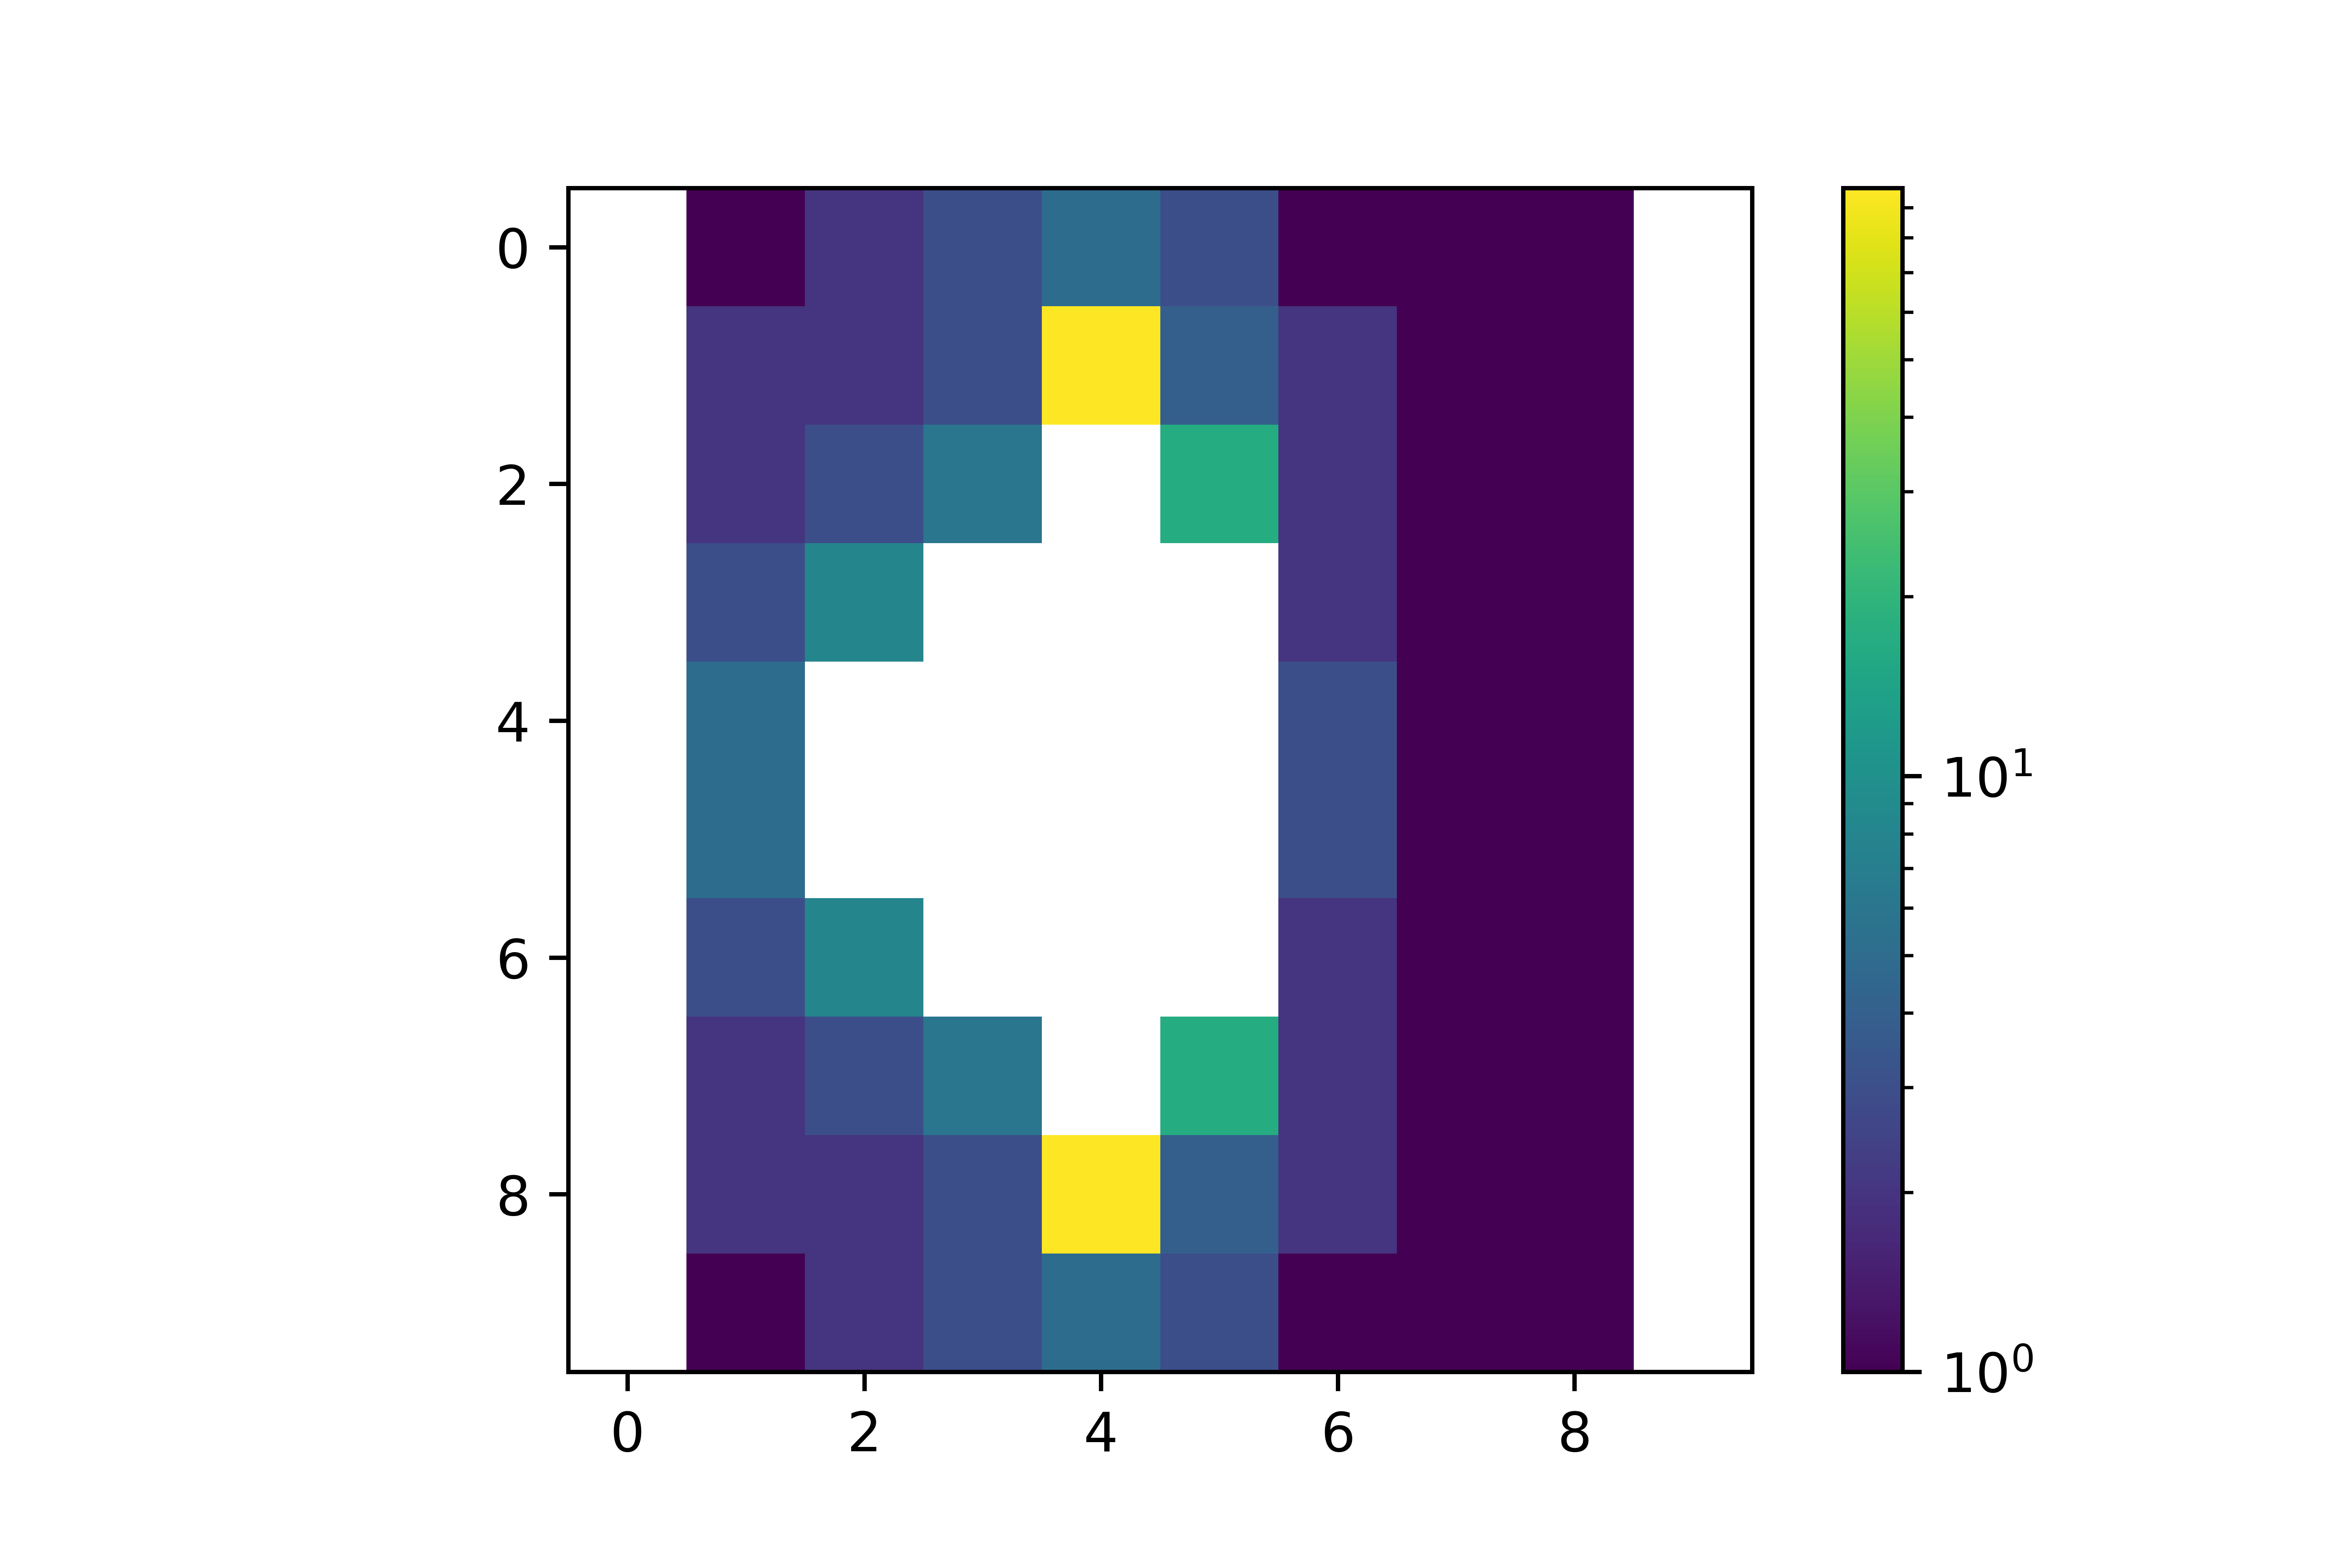
\includegraphics[width=\textwidth]{Low.png}\hfill
                        \caption{10x10 resolution}
                        \label{fig:low-res}
                        \end{subfigure}
                        \hfill
                        \begin{subfigure}[b]{0.47\textwidth}
                            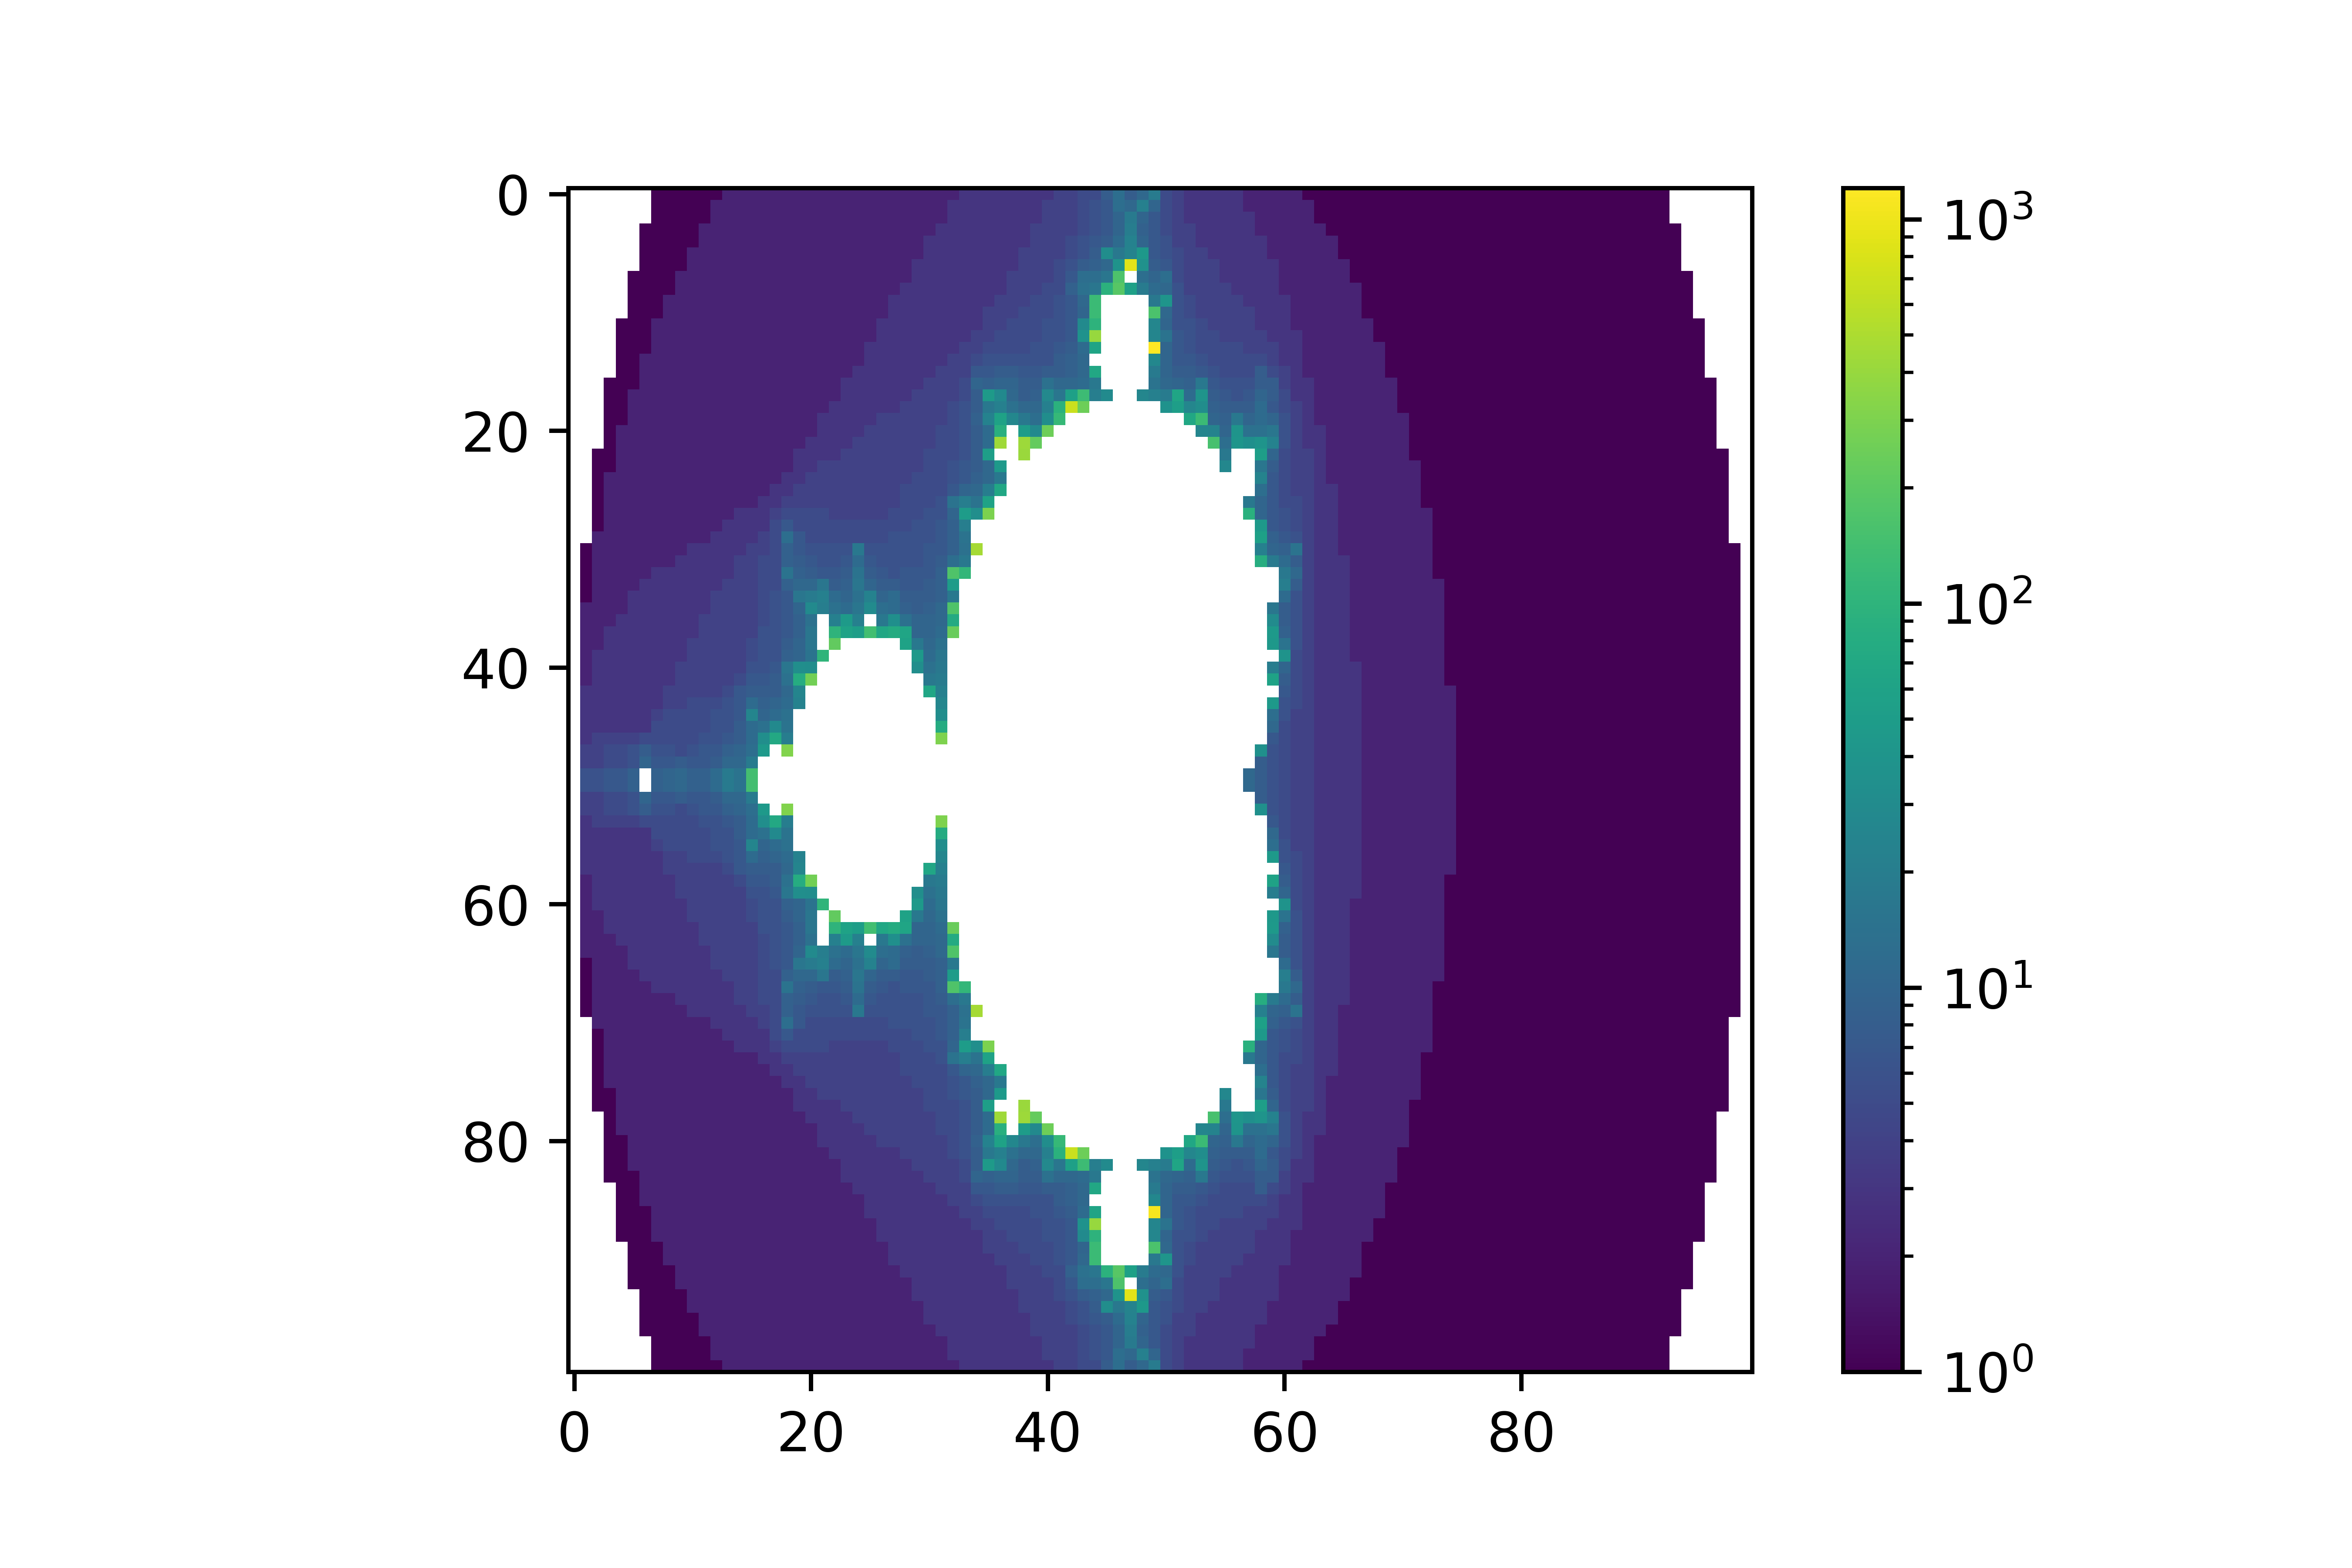
\includegraphics[width=\textwidth]{Mid.png}\hfill
                            \caption{100x100 resolution}
                            \label{fig:mid-res}
                        \end{subfigure}

                        \begin{subfigure}[b]{0.47\textwidth}
                            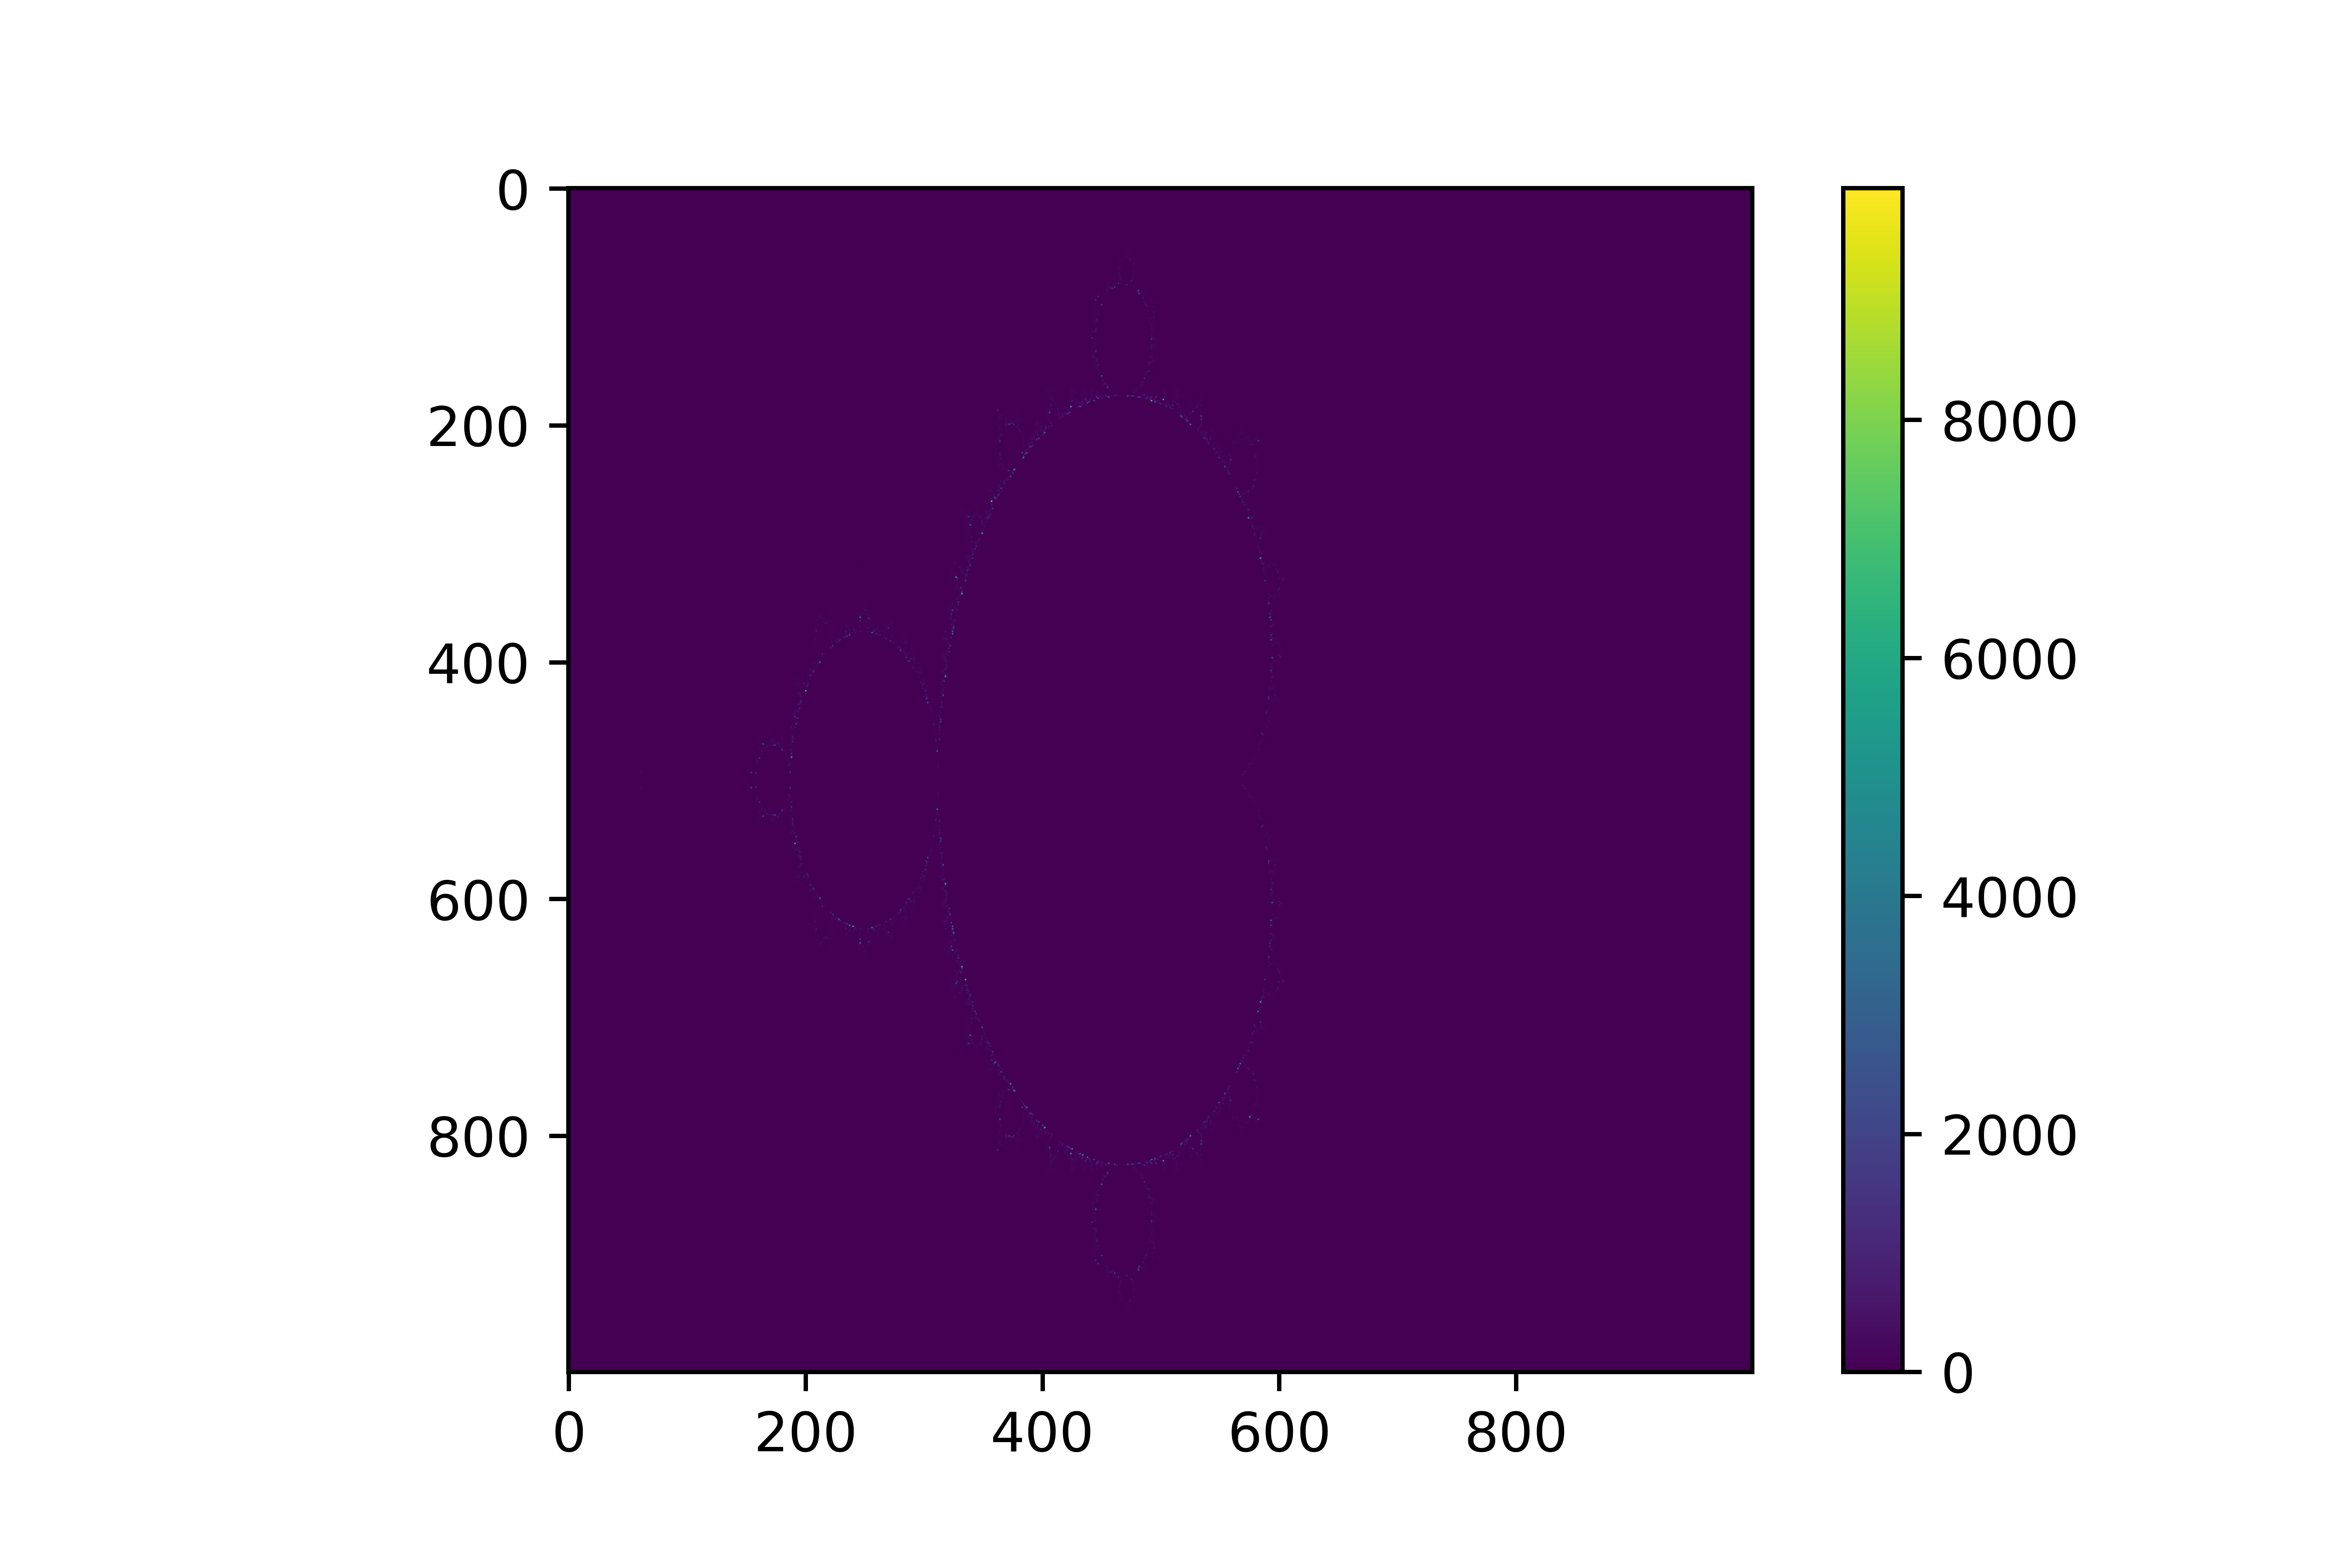
\includegraphics[width=\textwidth]{Linear_Scale.png}\hfill
                            \caption{1000x1000 Linear}
                            \label{fig:lin-res}
                        \end{subfigure}
                        \hfill
                        \begin{subfigure}[b]{0.47\textwidth}
                            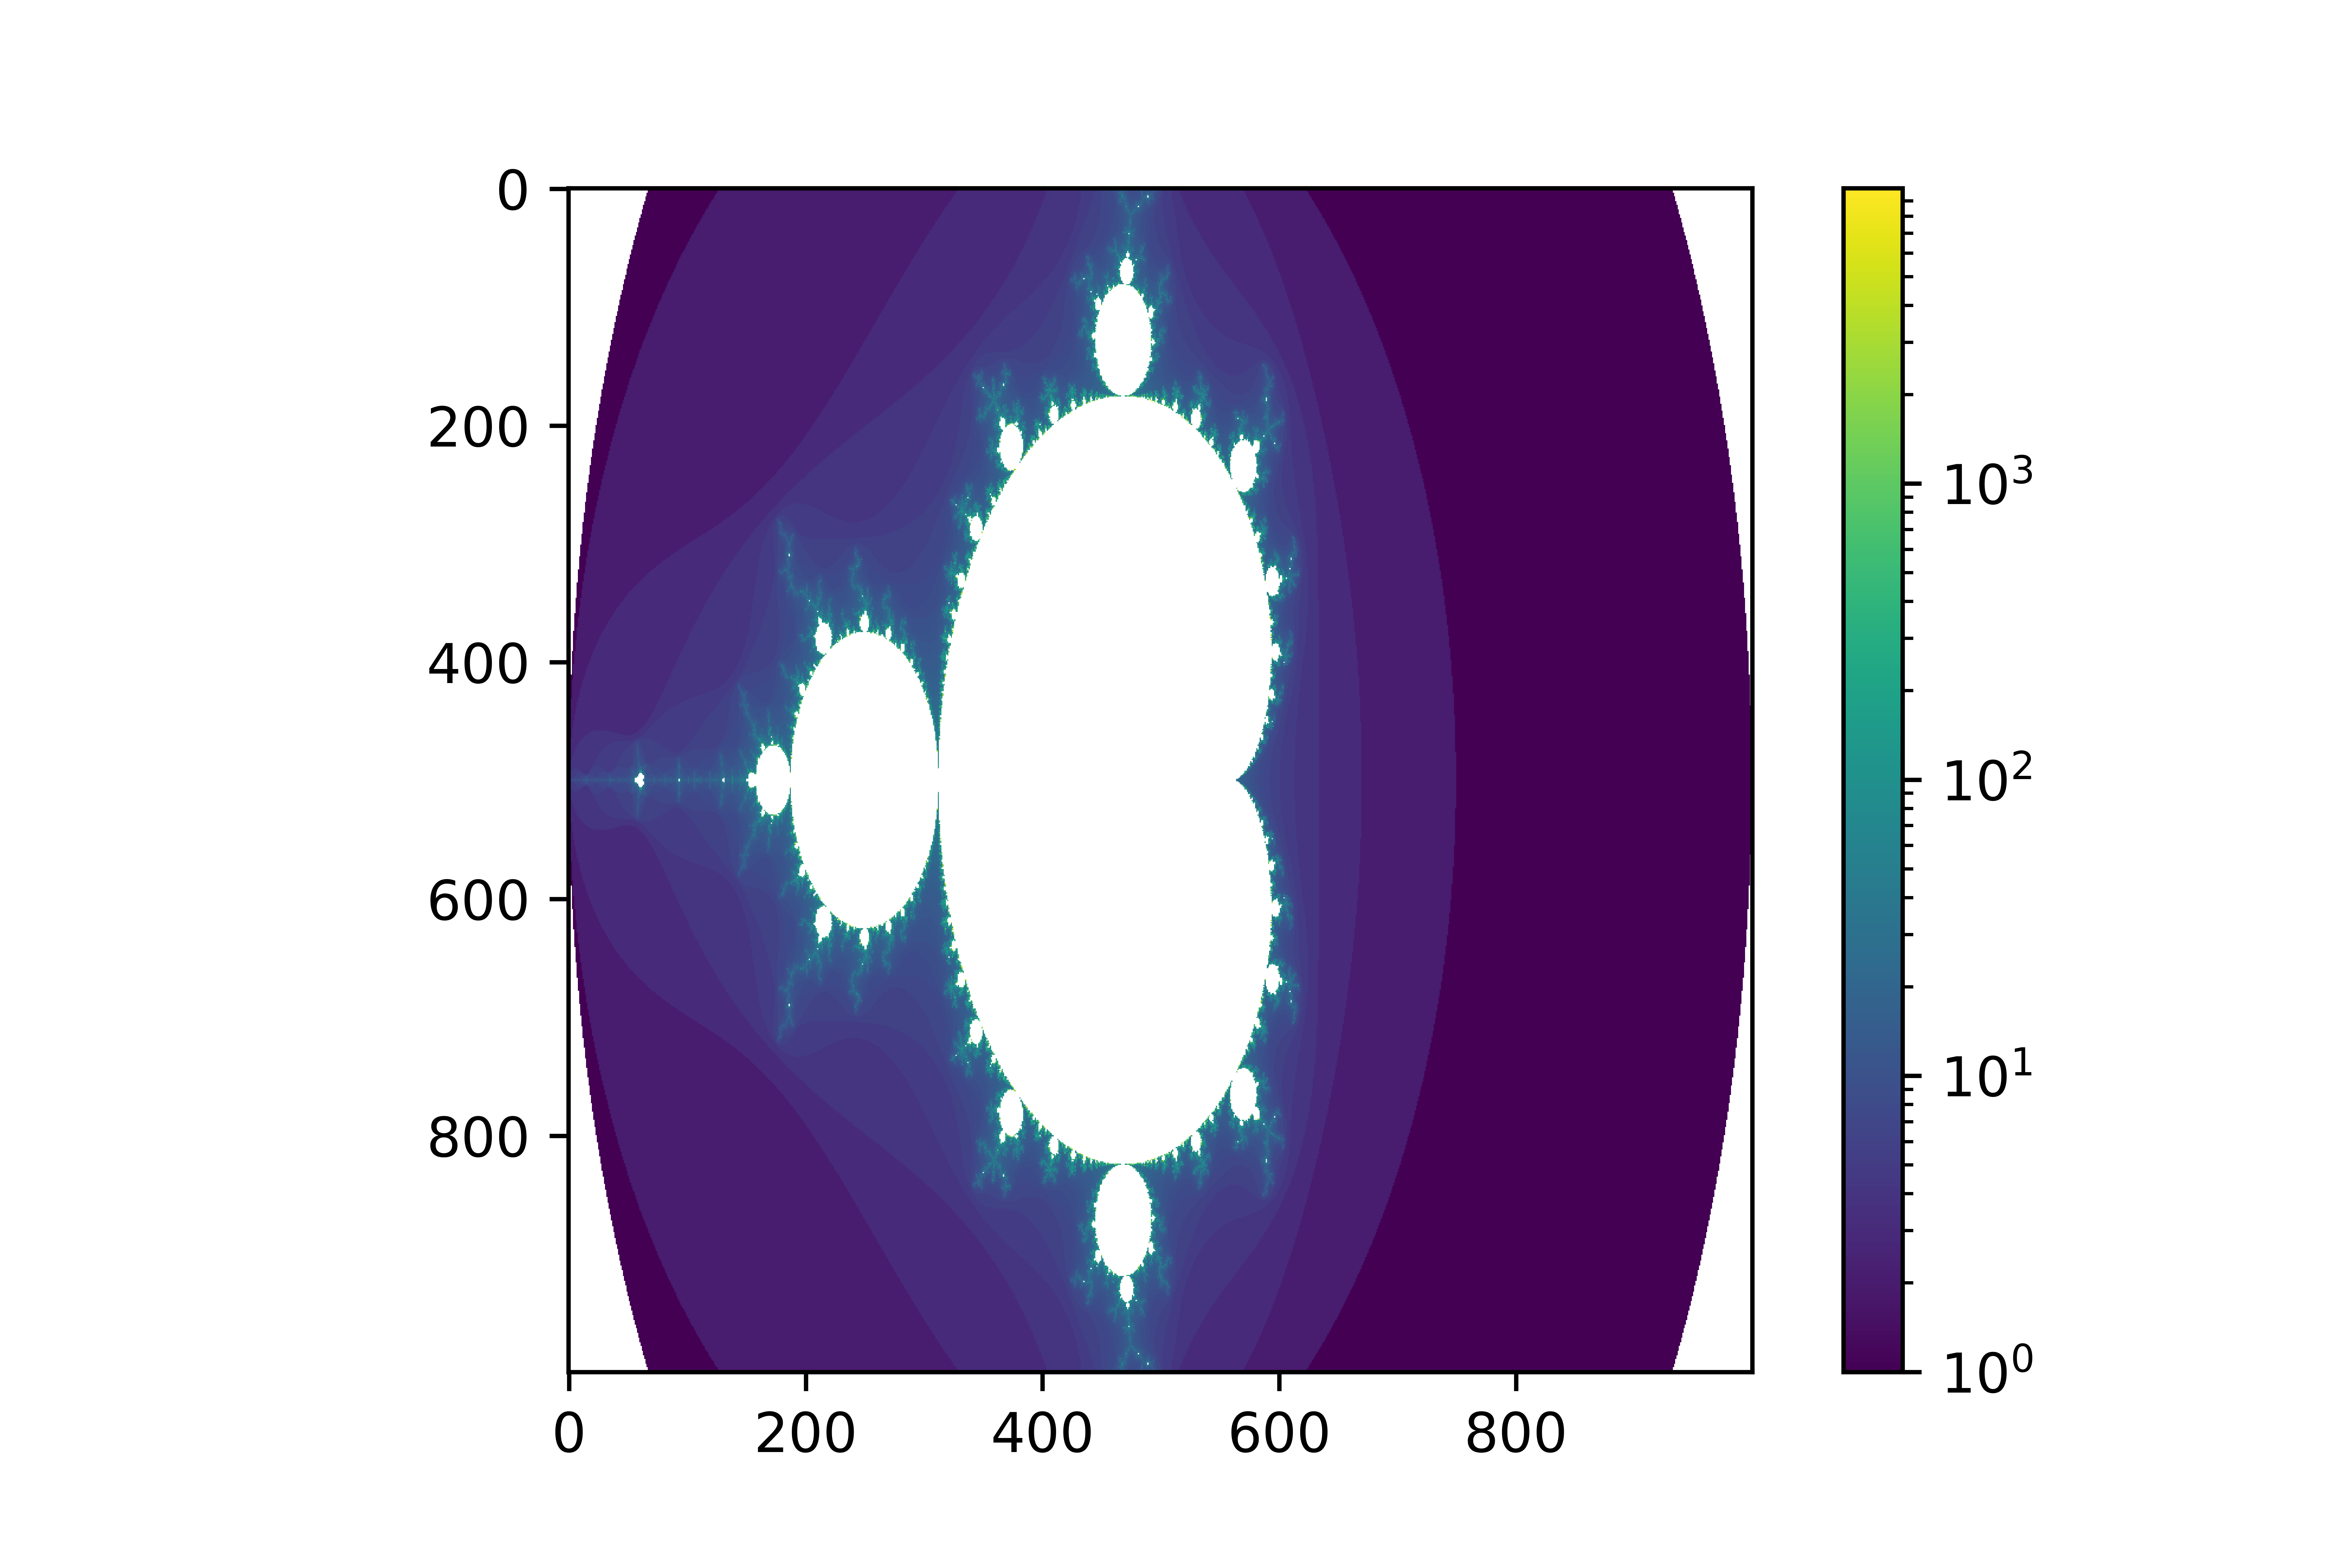
\includegraphics[width=\textwidth]{High.png}\hfill
                            \caption{1000x1000 resolution}
                            \label{fig:high-res}
                        \end{subfigure}
                \end{figure}

                In these images the white corresponds to a convergent pixel. While at the low resolution there is some resemblance to the general shape of the MB series, as the grid resolution increases more details of the fractal come into focus. As soon as the mid resolution the more detailed fine structures of the MB set can be seen. At the high resolution the image has take its iconic look. The images were plotted on a logarithmic color scale. There are several points along the ``edge'' of the fractal pattern that take several thousand iterations to converge. As a result the linear color scale plot is flat and uninformative. This is becasue the majority of points converge within a couple hundred iterations. The area calculations showed that as the resolution increased the area decreased and converged towards 1.86 units.


                \begin{center}
                \begin{tikzpicture}
                    \begin{axis}[
                        xmode=log,
                        log ticks with fixed point,
                        xlabel={Resolution (pixels)},
                        ylabel={Area}
                    ]
                    \addplot table {
                    10 2.880
                    100 1.910
                    1000 1.859
                    };
                    \end{axis}
                    \end{tikzpicture}
                \end{center}


        \end{enumerate}
        
    \section*{\label{sec:prob3} Problem 3}

        
        \begin{gather*}
            \text{let  } avg = \frac{\text{average cycles}}{\text{word access}} = f_c \times \frac{\text{cache cycles}}{\text{word access}} + (1-f_c) \frac{\text{main memory cycles}}{\text{word access}} \\ 
            \\
            \text{FLOPS} = \frac{2.3\text{GHz } \rho_{wm}}{avg} 
            \\
            \text{units:  } \frac{\text{\( \cancel{cycles}\)}}{s} \frac{flop}{\text{\( \cancel{word access} \)}} \frac{\text{\( \cancel{word access} \)}}{\text{\( \cancel{cycles}\)}}
        \end{gather*}

        Rearranging all the equations and plugging in given constants we get a final equation as seen below.
        \begin{gather*}
            \text{FLOPS} = \frac{2\times 2.3\mathrm{E}{-10}}{2f_c+100(1-f_c)}\frac{flop}{s}
        \end{gather*}
        The answers will be given without showing the plugin step.

        \begin{enumerate}
            \item $6.66\mathrm{E}{8}~\frac{flop}{s}$ 
            \item $9.02\mathrm{E}{7}~\frac{flop}{s}$
            \item $4.84\mathrm{E}{7}~\frac{flop}{s}$
            \item Plot given below.
            


            \begin{center}
                \begin{tikzpicture}
                    \begin{axis}[
                        enlargelimits=true,
                        ymode=log,
                        log ticks with fixed point,
                        xlabel={\% cache hits rate},
                        ylabel={FLOPS},
                        xmin=0, xmax=100,
                        ymin=0, ymax= 1000000000
                    ]
                    \addplot table[col sep=comma,row sep=crcr] {
                        5, 48400000 \\
                        50, 90200000 \\
                        95, 666000000 \\
                    };
                    \end{axis}
                    \end{tikzpicture}
                \end{center}

            \item  The system with 95\% cache hit rate has the best performance. It is able to complete an order of magnitude more floating point operations per second than the 50\% cache hit rate system.
            
        \end{enumerate}

        
    \section*{\label{sec:prob4} Problem 4}

    \begin{enumerate}
        \item L1 cache $<$ L2 cache $<$ main memory
        \item main memory $<$ L2 cache $\leq$ L1 cache
        \item Let us think of data as water that needs to be transported. If we work with the assumption that all water being transported is moving at a \textbf{constant} rate we can look at latency and bandwidth as properties of an empty pipe that transports the water. Latency is the length of the pipe from your starting point to your end point. The longer the pipe is the longer the delay till water starts flowing out the end point. So low latency means your data gets moved faster. On the other hand bandwidth is akin to the width of the pipe. A larger pipe can transport \textbf{more} water over the same length of pipe. This makes it so that even if you have a large latency you can still transfer a lot of data/water. \\
        Low latency and high bandwidth would give the fastest performance. In practice this can be difficult to achieve.
    \end{enumerate}


\end{document}
